% EVIDENCE-MANAGED-FILE
% VISUAL-MANAGED-FILE
% Numerical cells are generated; evidence status and identities stay in comments.
\IfFileExists{../output/exhibits/provisional_results_deck_values.tex}{%
% Generated by scripts/tabulate/render_provisional_results_deck_values.py.
% PROVISIONAL working-paper values; scientific identity is recorded in the provenance sidecar.
\newcommand{\StableCountBase}{16.9\%}
\newcommand{\StableCountEnd}{42.3\%}
\newcommand{\StableCountChange}{$+25.4$ pp}
\newcommand{\StableCountSE}{1.05 pp}
\newcommand{\StableCountP}{$3.35\times10^{-87}$}
\newcommand{\StableValueBase}{32.7\%}
\newcommand{\StableValueEnd}{76.5\%}
\newcommand{\StableValueChange}{$+43.9$ pp}
\newcommand{\StableValueSE}{2.02 pp}
\newcommand{\StableValueP}{$4.46\times10^{-75}$}
\newcommand{\MultiLegCountBase}{44.5\%}
\newcommand{\MultiLegCountEnd}{60.7\%}
\newcommand{\MultiLegCountChange}{$+16.3$ pp}
\newcommand{\MultiLegCountSE}{1.86 pp}
\newcommand{\MultiLegValueBase}{47.3\%}
\newcommand{\MultiLegValueEnd}{83.2\%}
\newcommand{\MultiLegValueChange}{$+35.9$ pp}
\newcommand{\MultiLegValueSE}{1.68 pp}
\newcommand{\WeakestComplexityCountChange}{$+17.0$ pp}
\newcommand{\WeakestComplexityCountSE}{1.36 pp}
\newcommand{\WeakestComplexityValueChange}{$+25.6$ pp}
\newcommand{\WeakestComplexityValueSE}{1.52 pp}
\newcommand{\JointStableContribution}{92.1\%}
\newcommand{\USDTCountExcessBase}{1.06}
\newcommand{\USDTCountExcessEnd}{1.23}
\newcommand{\USDTValueExcessBase}{0.59}
\newcommand{\USDTValueExcessEnd}{1.42}
\newcommand{\USDTCrossCountChange}{$+7.59$ pp}
\newcommand{\USDTCrossCountSE}{0.88 pp}
\newcommand{\USDTCrossValueChange}{$+12.00$ pp}
\newcommand{\USDTCrossValueSE}{2.03 pp}
\newcommand{\USDTEndpointGapBase}{$-7.13$ pp}
\newcommand{\USDTEndpointGapEnd}{$+8.14$ pp}
\newcommand{\USDTEndpointGapChange}{$+15.27$ pp}
\newcommand{\USDTEndpointGapSE}{1.50 pp}
\newcommand{\FullIntermediationBase}{13.95\%}
\newcommand{\FullIntermediationEnd}{11.92\%}
\newcommand{\FullIntermediationChange}{$-2.03$ pp}
\newcommand{\FullIntermediationSE}{0.39 pp}
\newcommand{\BalancedIntermediationEnd}{8.60\%}
\newcommand{\BalancedIntermediationChange}{$-5.35$ pp}
\newcommand{\BalancedIntermediationSE}{0.38 pp}
\newcommand{\CrossVenueCountStart}{2.0\%}
\newcommand{\CrossVenueCountEnd}{57.2\%}
\newcommand{\CrossVenueValueEnd}{79.1\%}
\newcommand{\CrossVenueRotationPremium}{$+7.45$ pp}
\newcommand{\CrossVenueRotationSE}{1.33 pp}
\newcommand{\VenueAllStableCountBase}{1.27}
\newcommand{\VenueAllStableCountEnd}{1.41}
\newcommand{\VenueAllStableValueBase}{0.84}
\newcommand{\VenueAllStableValueEnd}{1.24}
\newcommand{\VenueCPStableCountBase}{1.28}
\newcommand{\VenueCPStableCountEnd}{1.42}
\newcommand{\VenueCPStableValueBase}{0.78}
\newcommand{\VenueCPStableValueEnd}{1.33}
\newcommand{\VenueCPNativeValueEnd}{0.62}
\newcommand{\VenueAllStableValueChange}{$+0.40$}
\newcommand{\VenueCPStableValueChange}{$+0.55$}
\newcommand{\VenueCPEpisodeShare}{84.8\%}
\newcommand{\VenueBalancerPeakEpisodes}{39,536}
\newcommand{\VenueCPPeakEpisodes}{8,767,213}
\newcommand{\RouterWindowDays}{60}
\newcommand{\RouterReleaseCount}{3}
\newcommand{\RouterIntermediationBase}{20.8\%}
\newcommand{\RouterIntermediationEnd}{12.5\%}
\newcommand{\RouterIntermediationOne}{$-5.7$ pp}
\newcommand{\RouterIntermediationTwo}{$+0.8$ pp}
\newcommand{\RouterIntermediationThree}{$-0.7$ pp}
\newcommand{\RouterLargestIntermediationRise}{$+0.8$ pp}
\newcommand{\RouterLargestLegMovement}{0.049}
\newcommand{\RouterCrossBase}{8.5\%}
\newcommand{\RouterCrossOne}{$+2.5$ pp}
\newcommand{\RouterCrossTwo}{$+3.1$ pp}
\newcommand{\RouterCrossThree}{$-2.0$ pp}
\newcommand{\RouterCrossEnd}{24.4\%}
%
}{}
\IfFileExists{../output/exhibits/vehicle_transition_pair_decomposition_deck_values.tex}{%
% Generated by scripts/build_vehicle_transition_pair_deck_values.py; do not edit.
\newcommand{\PairPooledBase}{16.9\%}
\newcommand{\PairPooledEnd}{42.5\%}
\newcommand{\PairPooledTotal}{+25.7\,pp}
\newcommand{\PairPooledReweight}{+8.6\,pp}
\newcommand{\PairPooledSupportMass}{-0.5\,pp}
\newcommand{\PairPooledExclusive}{+17.8\,pp}
\newcommand{\PairPooledWithin}{-0.1\,pp}
\newcommand{\PairPooledBaseRawPct}{16.865562569}
\newcommand{\PairPooledEndRawPct}{42.540936227}
\newcommand{\PairPooledReweightRawPP}{8.572531324}
\newcommand{\PairPooledSupportMassRawPP}{-0.536299548}
\newcommand{\PairPooledExclusiveRawPP}{17.767073765}
\newcommand{\PairPooledWithinRawPP}{-0.127931883}
\newcommand{\PairSingleTotal}{+21.1\,pp}
\newcommand{\PairSingleWithin}{-0.3\,pp}
\newcommand{\PairCrossTotal}{+31.4\,pp}
\newcommand{\PairCrossWithin}{-0.3\,pp}
\newcommand{\PairValueTotal}{+42.8\,pp}
\newcommand{\PairValueWithin}{0.0\,pp}
\newcommand{\PairValueReweight}{+26.2\,pp}
\newcommand{\PairValueSupportMass}{-2.5\,pp}
\newcommand{\PairValueExclusive}{+19.2\,pp}
%
}{\PackageError{dvc-deck}{Missing generated vehicle-pair decomposition values}{Run scripts/build_vehicle_transition_pair_deck_values.py.}}
\IfFileExists{../output/exhibits/v1_architecture_deck_values.tex}{%
% Generated presentation binding for the admitted V1/V2 architecture result.
% Source: docs/finding-v1-forced-vehicle.md at ebeb23cf56b15dc78d798ea5770976560384a6d0.
% The regression in tests/test_deck_evidence.py reopens these bindings against
% the source tables whenever either file changes.
\newcommand{\VOneForcedRoutes}{217,003}
\newcommand{\VTwoWethTradeShare}{95.5\%}
\newcommand{\VTwoWethNewPairShare}{97.9\%}
%
}{\PackageError{dvc-deck}{Missing generated V1/V2 architecture values}{Rebuild the admitted V1/V2 presentation binding.}}

% EVIDENCE-STATUS: evolving route result; current certified route release
% EVIDENCE-COMMIT: 2ffbce0
% EVIDENCE-SOURCES: output/figures/experiments/annual_vehicle_composition_bands.pdf; output/exhibits/intermediation_by_type.jsonl; docs/findings-freeze.md
% VISUAL-FUNCTION: non-monotone realised vehicle rotation | annual native/stable lead comparison separated by count/value | expose the value lead-loss-retake path without implying treatment
\begin{frame}{Stablecoins regain the lead in routed value}
\vspace{-0.05cm}
\begin{center}
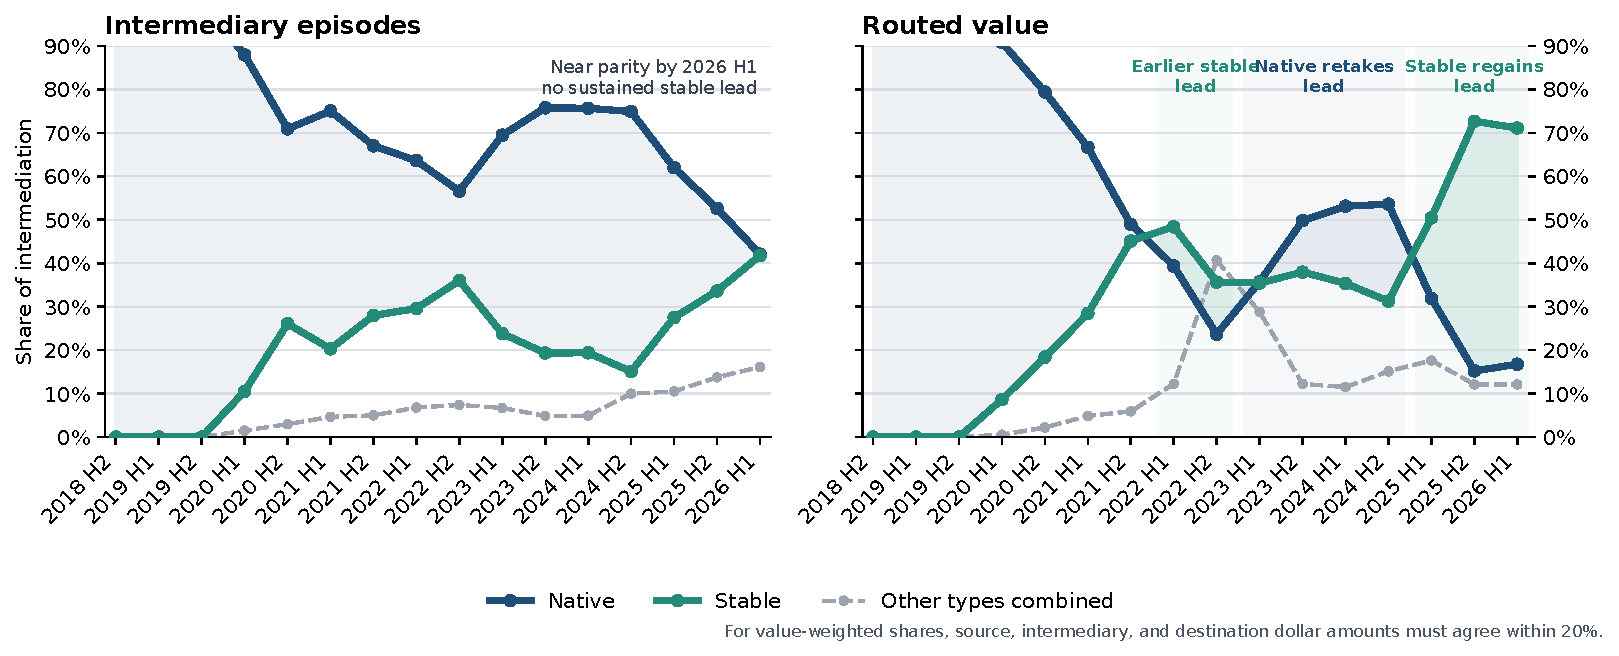
\includegraphics[width=0.94\textwidth,height=0.69\textheight,keepaspectratio]{../output/figures/experiments/annual_vehicle_composition_bands.pdf}
\end{center}
\vspace{-0.14cm}
\decknote{Annual shares of observed vehicle routes. The 2026 observation covers January--June; Other combines imported, liquid-staking, and residual assets.}
\end{frame}

% EVIDENCE-STATUS: evolving route decomposition; venue-scope reweighting is a route-only descriptive identity
% EVIDENCE-COMMIT: 6dd7897
% EVIDENCE-SOURCES: output/figures/vehicle_excess_use_transition.pdf; output/exhibits/vehicle_excess_use.jsonl; output/exhibits/vehicle_excess_use_transition.jsonl; output/exhibits/e0_usdt_integration_decomposition.jsonl; docs/findings-freeze.md
% VISUAL-FUNCTION: candidate-level excess-use change | paired count/value dumbbells | identify the distinct USDT contribution
\begin{frame}{USDT drives the rise in stablecoin intermediation}
\vspace{-0.08cm}
\begin{center}
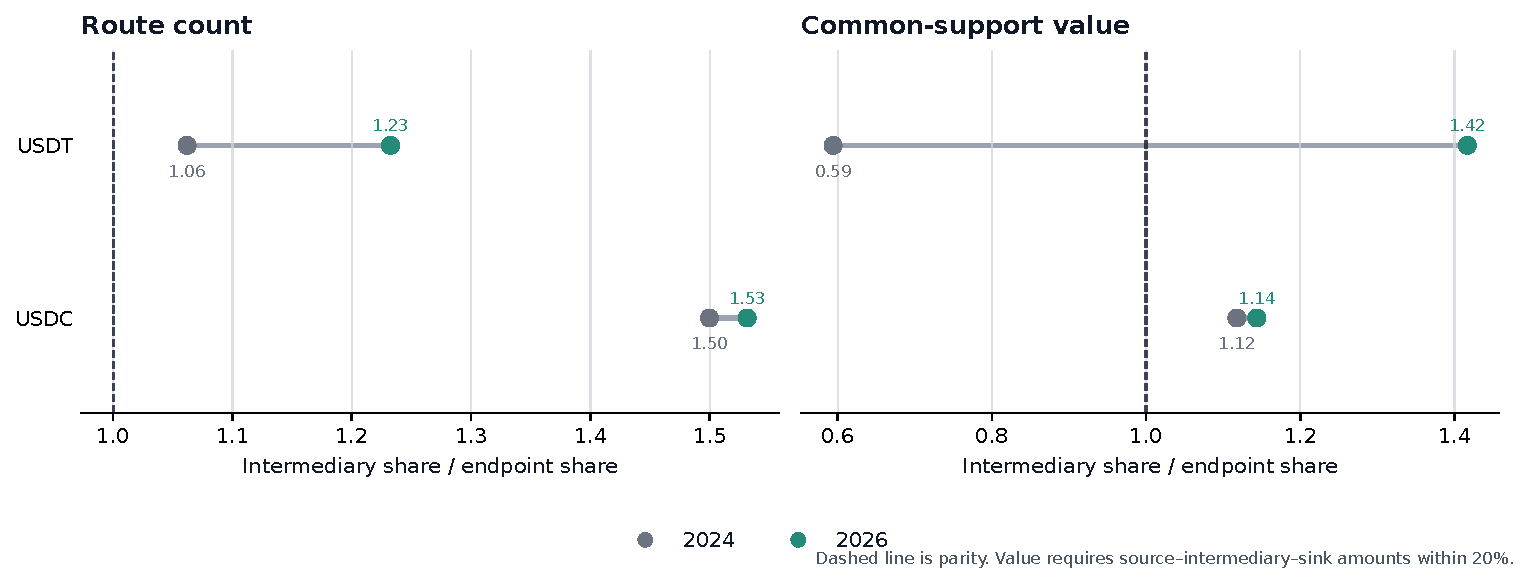
\includegraphics[width=0.93\textwidth,height=0.44\textheight,keepaspectratio]{../output/figures/vehicle_excess_use_transition.pdf}
\end{center}
\vspace{-0.16cm}
{\fontsize{6.8}{7.5}\selectfont USDT crosses parity by routed value and extends its count advantage; USDC changes little.}
\vspace{0.04cm}
\begin{beamercolorbox}[sep=0.08cm,wd=\textwidth]{block body}
{\fontsize{7.0}{7.7}\selectfont\bfseries \USDTVenueWithinCountShare{} of the count-share change and \USDTVenueWithinValueShare{} of the routed-value change occur within the single- and cross-venue categories.}
\end{beamercolorbox}
\decknote{Excess use is intermediary share divided by endpoint share on the same route perimeter. The comparison uses the same January--June dates in 2024 and 2026.}
\end{frame}

% EVIDENCE-STATUS: certified descriptive route accounting and matched-market estimate; mechanism remains open
% EVIDENCE-COMMIT: b21ed0a
% EVIDENCE-PRODUCER-COMMIT: 0f90441
% EVIDENCE-SOURCES: output/exhibits/vehicle_transition_pair_decomposition.jsonl; output/exhibits/vehicle_transition_pair_support.jsonl; output/exhibits/vehicle_transition_pair_fixed_effects.jsonl; output/exhibits/vehicle_transition_pair_decomposition_deck_values.tex
% VISUAL-FUNCTION: five-factor composition plus matched-market confidence interval | native TikZ accounting ribbon and interval | distinguish observed pair support, activity, vehicle incidence, and within-market stable-share change
\begin{frame}{Pair activity and vehicle use: \PairAndVehicleShare{} of the gain}
\vspace{-0.34cm}
\begin{center}
\resizebox{0.93\textwidth}{!}{% Presentation geometry only. Numerical labels are generated in
% output/exhibits/route_methodology_heterogeneity_deck_values.tex.
% WETH is the native intermediary in this comparison. If WETH is an endpoint,
% it cannot also be the intermediary; every such row therefore has stable_share=1.
\begin{tikzpicture}[x=1cm,y=1cm]
\tikzset{panel/.style={draw=rule,fill=white,rounded corners=3pt,line width=0.8pt}}
\tikzset{small/.style={font=\fontsize{6.8}{7.5}\selectfont,text=muted,align=center}}

\node[draw=stable,line width=1.1pt,circle,minimum size=1.05cm,
  font=\fontsize{8.2}{8.8}\selectfont\bfseries,text=ucldark] at (1.05,3.45) {WETH};
\node[anchor=west,font=\fontsize{8.2}{9.0}\selectfont\bfseries,text=ucldark]
  at (1.82,3.62) {WETH is an endpoint of the ultimate pair};
\node[anchor=west,font=\fontsize{7.2}{8.0}\selectfont,text=ink]
  at (1.82,3.25) {Stablecoins alone remain eligible as intermediaries.};

\draw[panel] (0,0.56) rectangle (6.00,2.68);
\node[anchor=west,font=\fontsize{8.1}{8.8}\selectfont\bfseries,text=ucldark]
  at (0.35,2.32) {All matched ultimate-pair groups};
\node[anchor=west,font=\fontsize{23}{24}\selectfont\bfseries,text=stable]
  at (0.35,1.48) {\WethCountFullChange};
\node[anchor=west,font=\fontsize{6.9}{7.6}\selectfont,text=muted]
  at (0.35,1.05) {95\% CI [\WethCountFullCILower, \WethCountFullCIUpper]};
\node[anchor=west,font=\fontsize{7.0}{7.7}\selectfont,text=ink]
  at (0.35,0.80) {WETH-linked route-count mass: \WethCountMassBase{} $\rightarrow$ \WethCountMassEnd};

\draw[panel] (6.35,0.56) rectangle (12.35,2.68);
\node[anchor=west,font=\fontsize{8.1}{8.8}\selectfont\bfseries,text=ucldark]
  at (6.70,2.32) {Ultimate-pair groups excluding WETH endpoints};
\node[anchor=west,font=\fontsize{23}{24}\selectfont\bfseries,text=accent]
  at (6.70,1.48) {\WethCountNoEndpointChange};
\node[anchor=west,font=\fontsize{6.9}{7.6}\selectfont,text=muted]
  at (6.70,1.05) {95\% CI [\WethCountNoEndpointCILower, \WethCountNoEndpointCIUpper]};
\node[anchor=west,font=\fontsize{7.0}{7.7}\selectfont,text=ink]
  at (6.70,0.80) {\WethCountNoEndpointGroups{} matched groups};

\node[small,text width=12.0cm] at (6.18,0.08)
  {\textbf{Within-ultimate-pair change:} all groups \WethCountWithinFullChange{} [\WethCountWithinFullCILower, \WethCountWithinFullCIUpper];\\excluding WETH endpoints \WethCountWithinNoEndpointChange{} [\WethCountWithinNoEndpointCILower, \WethCountWithinNoEndpointCIUpper].};
\end{tikzpicture}
}
\end{center}
\vspace{-0.38cm}
{\fontsize{8.2}{9.1}\selectfont\textbf{Dollar-weighted routes show the same broad allocation.} Stable share rises \PairValueTotal, with \PairValueReweight\ from activity weights among continuing pairs and only \PairValueWithin\ from stable-for-native substitution within them.}

\vspace{0.02cm}
\decknote{The sample contains exact two-leg routes observed in 2024 and January--June 2026. Matched estimates compare the same ordered endpoint pair, calendar date, and single- versus cross-venue route category. Dollar-weighted calculations retain routes for which the source, intermediary, and destination dollar amounts agree within 20\%.}
\end{frame}

% EVIDENCE-STATUS: certified descriptive result; integration remains a selected route stratum
% EVIDENCE-COMMIT: a0c54e9
% EVIDENCE-SOURCES: output/figures/experiments/integration_change_forest.pdf; output/exhibits/intermediation_integration_rival.jsonl; output/exhibits/intermediation_integration_interaction.jsonl; docs/findings-freeze.md
% VISUAL-FUNCTION: integration-stratified vehicle rotation | change estimates with HAC intervals | test whether venue mix absorbs the stable-share change
\begin{frame}{Stablecoin use rises within each venue scope}
\vspace{-0.08cm}
\begin{center}
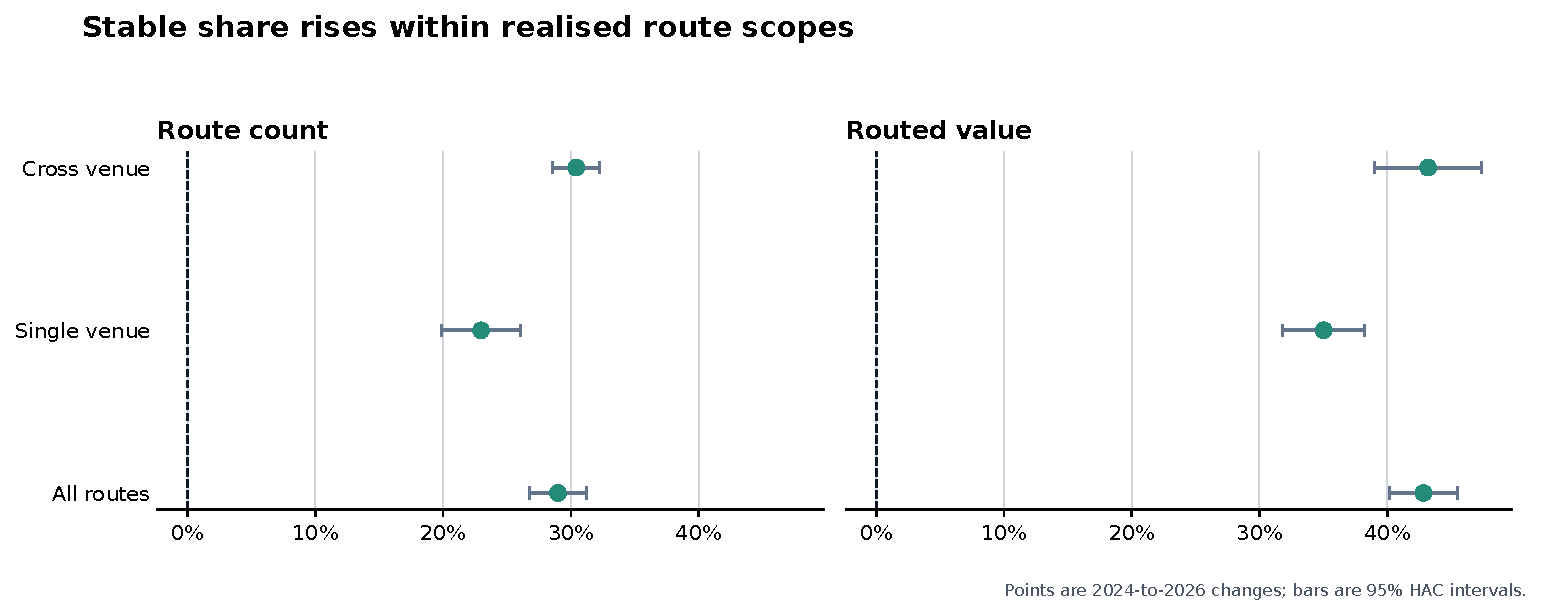
\includegraphics[width=0.89\textwidth,height=0.46\textheight,keepaspectratio]{../output/figures/experiments/integration_change_forest.pdf}
\end{center}
\vspace{-0.15cm}
{\fontsize{6.8}{7.5}\selectfont The increase appears within both realised route scopes, so a change in the single- versus cross-venue mix cannot account for the aggregate rotation. Cross-venue status remains selected; the comparison does not identify an effect of integration, routing software, or protocol architecture.}
\decknote{Changes compare the same January--June dates in 2024 and 2026. Bars show 95\% calendar-HAC confidence intervals.}
\end{frame}

% EVIDENCE-STATUS: registered mechanism design; no current LP estimate is displayed
% EVIDENCE-COMMIT: ab2c762
% EVIDENCE-SOURCES: docs/specification-lock.json; docs/findings-freeze.md; paper/sections/05-rivals.tex
% SCIENTIFIC-BOUNDARY: temporal ordering is not causal feedback; V2 capital stocks and V3 provider flows remain separate objects
% VISUAL-FUNCTION: liquidity timing test | two opposed timelines | distinguish capital-leading-use from use-leading-capital
\begin{frame}{Does liquidity move before vehicle use or follow it?}
\vspace{0.02cm}
\begin{columns}[T,totalwidth=\textwidth]
\begin{column}{0.48\textwidth}
\evidencekicker{Liquidity precedes use}
\vspace{0.25cm}
\centering
\begin{tikzpicture}[x=1cm,y=1cm]
\node[softbox,text width=4.35cm,minimum height=0.78cm,align=center] (capital) at (0,2.60) {More capital or provider inflow\\in vehicle-linked pools at $t$};
\node[softbox,text width=4.35cm,minimum height=0.78cm,align=center] (route) at (0,0.68) {More routes through the same vehicle\\at $t+\tau$};
\draw[-{Stealth[length=6pt]},line width=1.7pt,draw=stable] (capital)-- node[right,font=\scriptsize,text=muted] {predicts} (route);
\end{tikzpicture}
\par\vspace{0.10cm}\raggedright
{\small Liquidity supply may help a vehicle attract later routes.\par}
\end{column}
\begin{column}{0.48\textwidth}
\evidencekicker{Use precedes liquidity}
\vspace{0.25cm}
\centering
\begin{tikzpicture}[x=1cm,y=1cm]
\node[softbox,text width=4.35cm,minimum height=0.78cm,align=center] (route2) at (0,2.60) {More routes through a vehicle\\at $t$};
\node[softbox,text width=4.35cm,minimum height=0.78cm,align=center] (capital2) at (0,0.68) {More capital or provider inflow\\in its pools at $t+\tau$};
\draw[-{Stealth[length=6pt]},line width=1.7pt,draw=ucldark] (route2)-- node[right,font=\scriptsize,text=muted] {predicts} (capital2);
\end{tikzpicture}
\par\vspace{0.10cm}\raggedright
{\small Providers may instead follow routed demand.\par}
\end{column}
\end{columns}
\vspace{0.10cm}
{\fontsize{7.2}{8.0}\selectfont V2 capital stocks and V3 provider flows are tested separately at fixed lags; either ordering may reflect common demand or routing shocks.}
\end{frame}

% EVIDENCE-STATUS: registered V4 extension design; current estimate pending
% EVIDENCE-COMMIT: ab2c762
% EVIDENCE-SOURCES: docs/research-questions-and-empirical-design.md; docs/findings-freeze.md; paper/sections/05-rivals.tex
% SCIENTIFIC-BOUNDARY: settlement mechanics and route choice are distinct outcomes; launch date is not treatment
% VISUAL-FUNCTION: V4 settlement estimand | economic route versus physical transfer layers | show the matched comparison required to separate them
\begin{frame}{V4 separates the economic route from physical settlement}
\begin{columns}[T,totalwidth=\textwidth]
\begin{column}{0.48\textwidth}
\evidencekicker{Economic route}
\vspace{0.12cm}
\centering
\begin{tikzpicture}[x=1cm,y=1cm,tinyasset/.style={circle,draw=ink,fill=white,minimum size=23pt,inner sep=0pt,font=\small},routearrow/.style={-{Stealth[length=5pt]},line width=1.4pt}]
\node[tinyasset] (a) at (0,2.45) {A};
\node[tinyasset,fill=ucldark,text=white,draw=ucldark] (k) at (2.05,2.45) {$k$};
\node[tinyasset] (b) at (4.10,2.45) {B};
\draw[routearrow,draw=ucldark] (a)--(k);
\draw[routearrow,draw=ucldark] (k)--(b);
\node[anchor=north,align=center,font=\small,text width=5.2cm] at (2.05,1.82) {Pool calls route through intermediary $k$.};
\node[rounded corners=3pt,draw=uclbright,densely dashed,minimum width=5.0cm,minimum height=0.82cm,align=center,font=\scriptsize] at (2.05,0.45) {Prediction: fewer token transfers\\for comparable two-pool routes.};
\end{tikzpicture}
\end{column}
\begin{column}{0.05\textwidth}
\mbox{}
\end{column}
\begin{column}{0.44\textwidth}
\evidencekicker{Matched comparison}
\vspace{0.12cm}
{\scriptsize
\begin{itemize}
\setlength{\itemsep}{0.25em}
\item Compare routes in the same week, endpoint pair, intermediary, direction, and trade-size group.
\item Record route use and token transfers separately.
\item Compare feasible alternatives before interpreting vehicle choice.
\end{itemize}
}
\end{column}
\end{columns}
\end{frame}

% EVIDENCE-STATUS: diagnostic displacement gradient; not a persistence estimate
% EVIDENCE-COMMIT: 3873fca
% EVIDENCE-SOURCES: output/exhibits/provisional_results_deck_values.tex; docs/findings-freeze.md
% VISUAL-FUNCTION: 30-day challenger and incumbent share changes | coefficient table pending difference plot | expose direction, uncertainty, and risk-set limitation
\begin{frame}{Challenger cost advantage predicts subsequent vehicle share}
\vspace{0.18cm}
{\small
\begin{tabular}{@{}p{0.43\textwidth}rrr@{}}
\toprule
\textbf{30-day outcome} & $\hat\beta$ & \textbf{SE} & $t$ \\
\midrule
Change in challenger vehicle share & \ChallengerCoef & \ChallengerSE & \ChallengerT \\
Change in incumbent vehicle share & \IncumbentCoef & \IncumbentSE & \IncumbentT \\
Challenger leads after 30 days & \OvertakeCoef & \OvertakeSE & \OvertakeT \\
\bottomrule
\end{tabular}}
\vspace{0.25cm}

\decknote{$\hat\beta$ is the coefficient on the challenger's cost advantage. Outcomes are measured 30 days later. The sample contains $N=\DiagnosticN$ endpoint-pair--intermediary observations and \DiagnosticClusters\ date clusters; standard errors are clustered by date and use the CR1 rank correction.}
\vspace{0.36cm}
\begin{beamercolorbox}[sep=0.22cm,wd=\textwidth]{block body}
The estimates are large in the small set of endpoint markets and intermediary assets we can follow. They remain descriptive because the panel does not compare each market against a fixed set of feasible routes.
\end{beamercolorbox}
\end{frame}

% EVIDENCE-STATUS: admitted V1 mandate and V2 pair-formation result
% EVIDENCE-COMMIT: ebeb23c
% EVIDENCE-SOURCES: docs/finding-v1-forced-vehicle.md; output/exhibits/v1_forced_vehicle_report.md; output/exhibits/v1_architecture_deck_values.tex
% VISUAL-FUNCTION: architecture and persistence | V1-to-V2 mechanism comparison | show how imposed intermediation becomes endogenous pair formation
\begin{frame}{Native-asset pairing persists after it becomes optional}
\begin{columns}[T,totalwidth=\textwidth]
\begin{column}{0.43\textwidth}
\evidencekicker{V1: protocol rule}
\vspace{0.16cm}
\begin{tikzpicture}[x=1cm,y=1cm]
\node[nodepoint] (a) at (0.35,2.45) {A};
\node[nodepoint,fill=ucldark,text=white,draw=ucldark,minimum size=38pt] (eth) at (2.55,2.45) {ETH};
\node[nodepoint] (b) at (4.75,2.45) {B};
\draw[route,draw=accent,line width=1.7pt] (a)--(eth);
\draw[route,draw=accent,line width=1.7pt] (eth)--(b);
\node[font=\small\bfseries,text=ucldark,align=center] at (2.55,0.95) {\VOneForcedRoutes{} token-to-token trades\\pass through ETH};
\end{tikzpicture}
\vspace{0.10cm}
{\small Every token pool pairs with ETH, so the architecture imposes the vehicle.\par}
\end{column}
\begin{column}{0.08\textwidth}
\centering
\vspace{2.05cm}
{\Large$\Longrightarrow$}
\end{column}
\begin{column}{0.45\textwidth}
\evidencekicker{V2: market choice}
\vspace{0.20cm}
\begin{beamercolorbox}[sep=0.28cm,wd=\textwidth]{block body}
{\fontsize{24}{26}\selectfont\bfseries\color{ucldark}\VTwoWethTradeShare}\par
{\small of single-leg V2 trades use a WETH pool in 2026}
\end{beamercolorbox}
\vspace{0.26cm}
\begin{beamercolorbox}[sep=0.28cm,wd=\textwidth]{block body}
{\fontsize{24}{26}\selectfont\bfseries\color{stable}\VTwoWethNewPairShare}\par
{\small of pairs first traded in 2026 include WETH}
\end{beamercolorbox}
\end{column}
\end{columns}
\vspace{0.10cm}
{\small V2 converted ETH pairing from a protocol rule into a market choice. Native-asset concentration remained high through pair formation and realised trading.\par}
\decknote{V1 counts linked token-to-ETH and ETH-to-token swaps with matching ETH quantities in one transaction. V2 shares use single-leg Uniswap V2 trades and newly traded pairs; they describe that venue rather than market-wide vehicle dominance.}
\end{frame}
